\documentclass[1p]{elsarticle_modified}
%\bibliographystyle{elsarticle-num}

%\usepackage[colorlinks]{hyperref}
%\usepackage{abbrmath_seonhwa} %\Abb, \Ascr, \Acal ,\Abf, \Afrak
\usepackage{amsfonts}
\usepackage{amssymb}
\usepackage{amsmath}
\usepackage{amsthm}
\usepackage{scalefnt}
\usepackage{amsbsy}
\usepackage{kotex}
\usepackage{caption}
\usepackage{subfig}
\usepackage{color}
\usepackage{graphicx}
\usepackage{xcolor} %% white, black, red, green, blue, cyan, magenta, yellow
\usepackage{float}
\usepackage{setspace}
\usepackage{hyperref}

\usepackage{tikz}
\usetikzlibrary{arrows}

\usepackage{multirow}
\usepackage{array} % fixed length table
\usepackage{hhline}

%%%%%%%%%%%%%%%%%%%%%
\makeatletter
\renewcommand*\env@matrix[1][\arraystretch]{%
	\edef\arraystretch{#1}%
	\hskip -\arraycolsep
	\let\@ifnextchar\new@ifnextchar
	\array{*\c@MaxMatrixCols c}}
\makeatother %https://tex.stackexchange.com/questions/14071/how-can-i-increase-the-line-spacing-in-a-matrix
%%%%%%%%%%%%%%%

\usepackage[normalem]{ulem}

\newcommand{\msout}[1]{\ifmmode\text{\sout{\ensuremath{#1}}}\else\sout{#1}\fi}
%SOURCE: \msout is \stkout macro in https://tex.stackexchange.com/questions/20609/strikeout-in-math-mode

\newcommand{\cancel}[1]{
	\ifmmode
	{\color{red}\msout{#1}}
	\else
	{\color{red}\sout{#1}}
	\fi
}

\newcommand{\add}[1]{
	{\color{blue}\uwave{#1}}
}

\newcommand{\replace}[2]{
	\ifmmode
	{\color{red}\msout{#1}}{\color{blue}\uwave{#2}}
	\else
	{\color{red}\sout{#1}}{\color{blue}\uwave{#2}}
	\fi
}

\newcommand{\Sol}{\mathcal{S}} %segment
\newcommand{\D}{D} %diagram
\newcommand{\A}{\mathcal{A}} %arc


%%%%%%%%%%%%%%%%%%%%%%%%%%%%%5 test

\def\sl{\operatorname{\textup{SL}}(2,\Cbb)}
\def\psl{\operatorname{\textup{PSL}}(2,\Cbb)}
\def\quan{\mkern 1mu \triangleright \mkern 1mu}

\theoremstyle{definition}
\newtheorem{thm}{Theorem}[section]
\newtheorem{prop}[thm]{Proposition}
\newtheorem{lem}[thm]{Lemma}
\newtheorem{ques}[thm]{Question}
\newtheorem{cor}[thm]{Corollary}
\newtheorem{defn}[thm]{Definition}
\newtheorem{exam}[thm]{Example}
\newtheorem{rmk}[thm]{Remark}
\newtheorem{alg}[thm]{Algorithm}

\newcommand{\I}{\sqrt{-1}}
\begin{document}

%\begin{frontmatter}
%
%\title{Boundary parabolic representations of knots up to 8 crossings}
%
%%% Group authors per affiliation:
%\author{Yunhi Cho} 
%\address{Department of Mathematics, University of Seoul, Seoul, Korea}
%\ead{yhcho@uos.ac.kr}
%
%
%\author{Seonhwa Kim} %\fnref{s_kim}}
%\address{Center for Geometry and Physics, Institute for Basic Science, Pohang, 37673, Korea}
%\ead{ryeona17@ibs.re.kr}
%
%\author{Hyuk Kim}
%\address{Department of Mathematical Sciences, Seoul National University, Seoul 08826, Korea}
%\ead{hyukkim@snu.ac.kr}
%
%\author{Seokbeom Yoon}
%\address{Department of Mathematical Sciences, Seoul National University, Seoul, 08826,  Korea}
%\ead{sbyoon15@snu.ac.kr}
%
%\begin{abstract}
%We find all boundary parabolic representation of knots up to 8 crossings.
%
%\end{abstract}
%\begin{keyword}
%    \MSC[2010] 57M25 
%\end{keyword}
%
%\end{frontmatter}

%\linenumbers
%\tableofcontents
%
\newcommand\colored[1]{\textcolor{white}{\rule[-0.35ex]{0.8em}{1.4ex}}\kern-0.8em\color{red} #1}%
%\newcommand\colored[1]{\textcolor{white}{ #1}\kern-2.17ex	\textcolor{white}{ #1}\kern-1.81ex	\textcolor{white}{ #1}\kern-2.15ex\color{red}#1	}

{\Large $\underline{12n_{0013}~(K12n_{0013})}$}

\setlength{\tabcolsep}{10pt}
\renewcommand{\arraystretch}{1.6}
\vspace{1cm}\begin{tabular}{m{100pt}>{\centering\arraybackslash}m{274pt}}
\multirow{5}{120pt}{
	\centering
	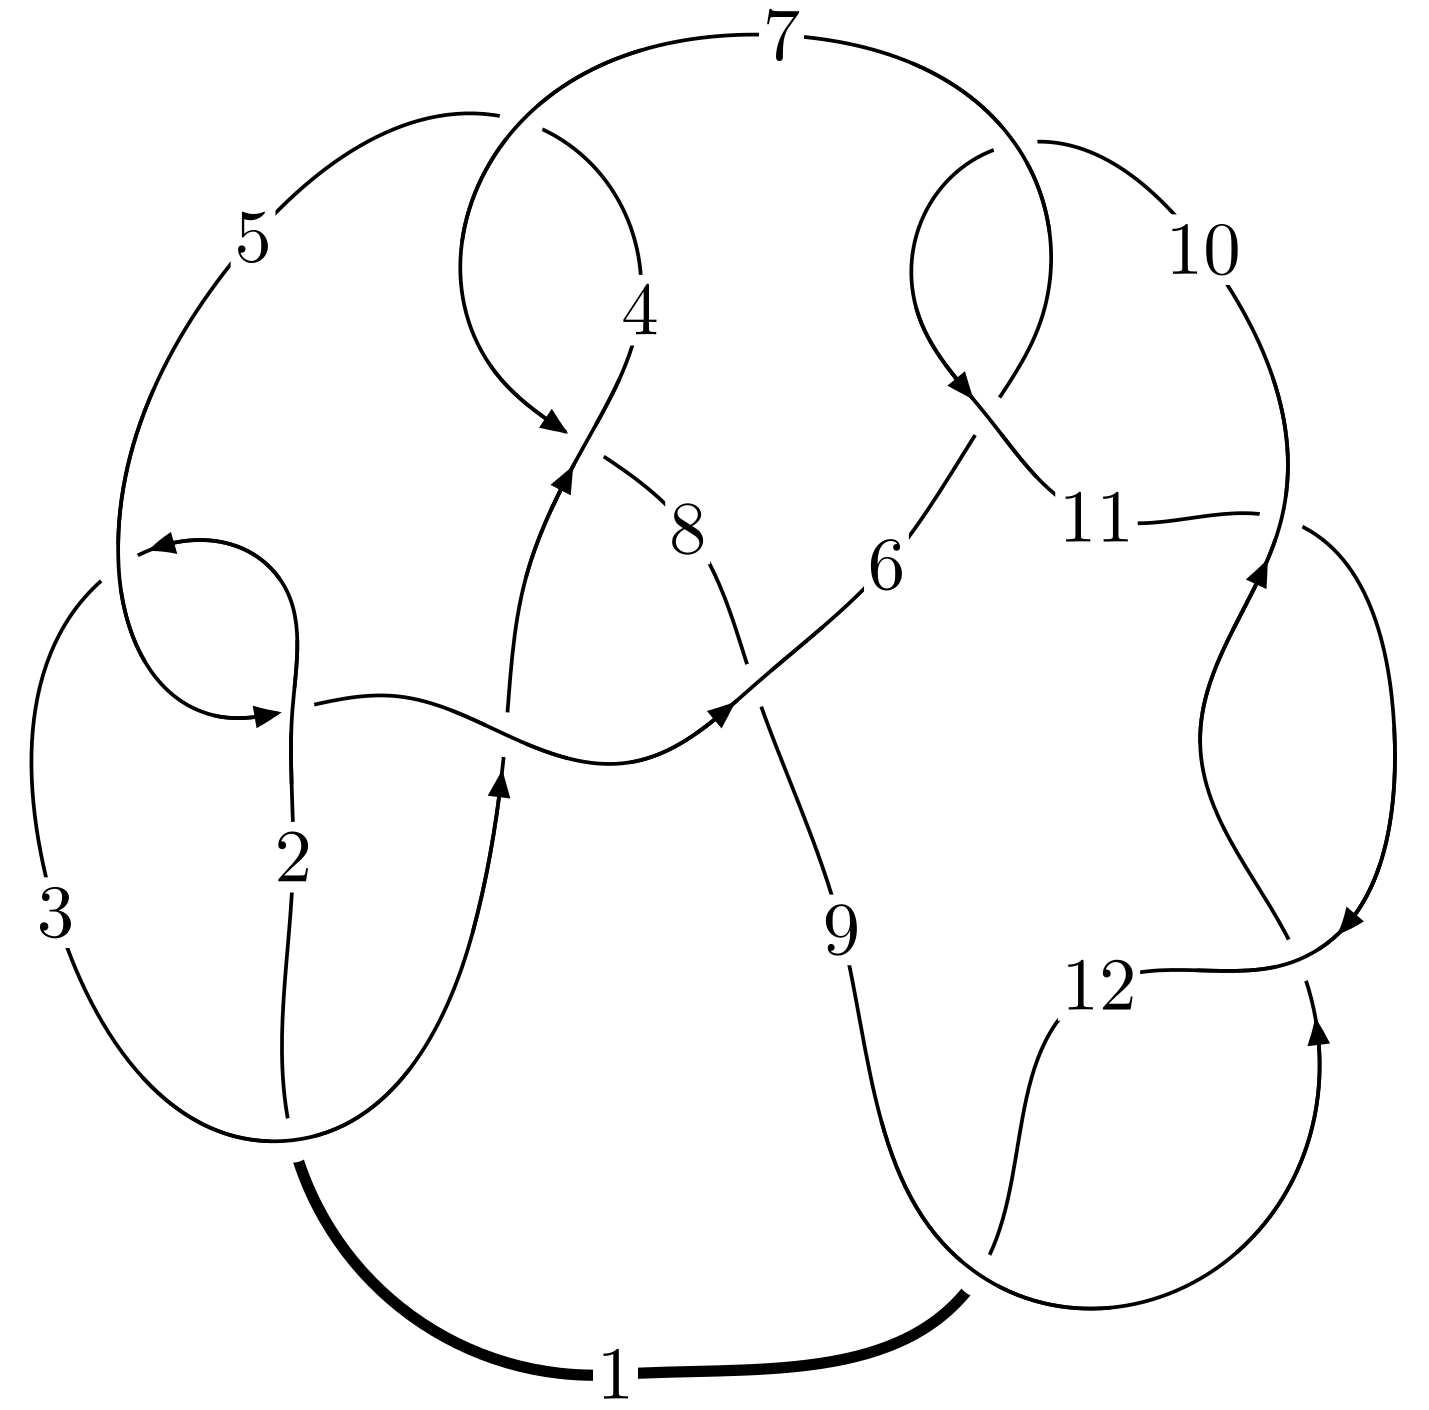
\includegraphics[width=112pt]{../../../GIT/diagram.site/Diagrams/png/2102_12n_0013.png}\\
\ \ \ A knot diagram\footnotemark}&
\allowdisplaybreaks
\textbf{Linearized knot diagam} \\
\cline{2-2}
 &
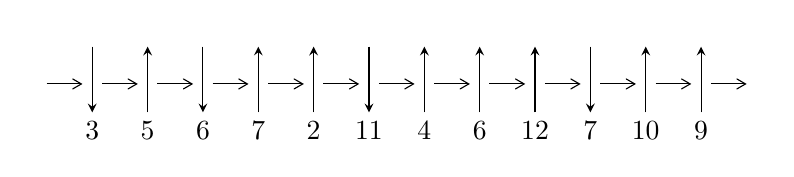
\begin{tikzpicture}[x=20pt, y=17pt]
	% nodes
	\node (C0) at (0, 0) {};
	\node (C1) at (1, 0) {};
	\node (C1U) at (1, +1) {};
	\node (C1D) at (1, -1) {3};

	\node (C2) at (2, 0) {};
	\node (C2U) at (2, +1) {};
	\node (C2D) at (2, -1) {5};

	\node (C3) at (3, 0) {};
	\node (C3U) at (3, +1) {};
	\node (C3D) at (3, -1) {6};

	\node (C4) at (4, 0) {};
	\node (C4U) at (4, +1) {};
	\node (C4D) at (4, -1) {7};

	\node (C5) at (5, 0) {};
	\node (C5U) at (5, +1) {};
	\node (C5D) at (5, -1) {2};

	\node (C6) at (6, 0) {};
	\node (C6U) at (6, +1) {};
	\node (C6D) at (6, -1) {11};

	\node (C7) at (7, 0) {};
	\node (C7U) at (7, +1) {};
	\node (C7D) at (7, -1) {4};

	\node (C8) at (8, 0) {};
	\node (C8U) at (8, +1) {};
	\node (C8D) at (8, -1) {6};

	\node (C9) at (9, 0) {};
	\node (C9U) at (9, +1) {};
	\node (C9D) at (9, -1) {12};

	\node (C10) at (10, 0) {};
	\node (C10U) at (10, +1) {};
	\node (C10D) at (10, -1) {7};

	\node (C11) at (11, 0) {};
	\node (C11U) at (11, +1) {};
	\node (C11D) at (11, -1) {10};

	\node (C12) at (12, 0) {};
	\node (C12U) at (12, +1) {};
	\node (C12D) at (12, -1) {9};
	\node (C13) at (13, 0) {};

	% arrows
	\draw[->,>={angle 60}]
	(C0) edge (C1) (C1) edge (C2) (C2) edge (C3) (C3) edge (C4) (C4) edge (C5) (C5) edge (C6) (C6) edge (C7) (C7) edge (C8) (C8) edge (C9) (C9) edge (C10) (C10) edge (C11) (C11) edge (C12) (C12) edge (C13) ;	\draw[->,>=stealth]
	(C1U) edge (C1D) (C2D) edge (C2U) (C3U) edge (C3D) (C4D) edge (C4U) (C5D) edge (C5U) (C6U) edge (C6D) (C7D) edge (C7U) (C8D) edge (C8U) (C9D) edge (C9U) (C10U) edge (C10D) (C11D) edge (C11U) (C12D) edge (C12U) ;
	\end{tikzpicture} \\
\hhline{~~} \\& 
\textbf{Solving Sequence} \\ \cline{2-2} 
 &
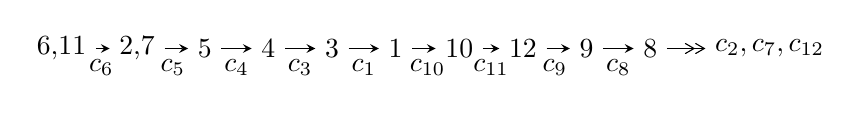
\begin{tikzpicture}[x=23pt, y=7pt]
	% node
	\node (A0) at (-1/8, 0) {6,11};
	\node (A1) at (17/16, 0) {2,7};
	\node (A2) at (17/8, 0) {5};
	\node (A3) at (25/8, 0) {4};
	\node (A4) at (33/8, 0) {3};
	\node (A5) at (41/8, 0) {1};
	\node (A6) at (49/8, 0) {10};
	\node (A7) at (57/8, 0) {12};
	\node (A8) at (65/8, 0) {9};
	\node (A9) at (73/8, 0) {8};
	\node (C1) at (1/2, -1) {$c_{6}$};
	\node (C2) at (13/8, -1) {$c_{5}$};
	\node (C3) at (21/8, -1) {$c_{4}$};
	\node (C4) at (29/8, -1) {$c_{3}$};
	\node (C5) at (37/8, -1) {$c_{1}$};
	\node (C6) at (45/8, -1) {$c_{10}$};
	\node (C7) at (53/8, -1) {$c_{11}$};
	\node (C8) at (61/8, -1) {$c_{9}$};
	\node (C9) at (69/8, -1) {$c_{8}$};
	\node (A10) at (11, 0) {$c_{2},c_{7},c_{12}$};

	% edge
	\draw[->,>=stealth]	
	(A0) edge (A1) (A1) edge (A2) (A2) edge (A3) (A3) edge (A4) (A4) edge (A5) (A5) edge (A6) (A6) edge (A7) (A7) edge (A8) (A8) edge (A9) ;
	\draw[->>,>={angle 60}]	
	(A9) edge (A10);
\end{tikzpicture} \\ 

\end{tabular} \\

\footnotetext{
The image of knot diagram is generated by the software ``\textbf{Draw programme}" developed by Andrew Bartholomew(\url{http://www.layer8.co.uk/maths/draw/index.htm\#Running-draw}), where we modified some parts for our purpose(\url{https://github.com/CATsTAILs/LinksPainter}).
}\phantom \\ \newline 
\centering \textbf{Ideals for irreducible components\footnotemark of $X_{\text{par}}$} 
 
\begin{align*}
I^u_{1}&=\langle 
- u^{20}+2 u^{19}+\cdots+3 u^2+2 b,\;- u^{20}+2 u^{19}+\cdots+2 a+1,\;u^{22}-3 u^{21}+\cdots- u+1\rangle \\
I^u_{2}&=\langle 
- u^3 a-2 u^2 a- u^3- a u-2 u^2+2 b- a- u-1,\;u^2 a+u^3+a^2+a u+u^2+2 a+u,\;u^4+u^3+u^2+1\rangle \\
\\
\end{align*}
\raggedright * 2 irreducible components of $\dim_{\mathbb{C}}=0$, with total 30 representations.\\
\footnotetext{All coefficients of polynomials are rational numbers. But the coefficients are sometimes approximated in decimal forms when there is not enough margin.}
\newpage
\renewcommand{\arraystretch}{1}
\centering \section*{I. $I^u_{1}= \langle - u^{20}+2 u^{19}+\cdots+3 u^2+2 b,\;- u^{20}+2 u^{19}+\cdots+2 a+1,\;u^{22}-3 u^{21}+\cdots- u+1 \rangle$}
\flushleft \textbf{(i) Arc colorings}\\
\begin{tabular}{m{7pt} m{180pt} m{7pt} m{180pt} }
\flushright $a_{6}=$&$\begin{pmatrix}1\\0\end{pmatrix}$ \\
\flushright $a_{11}=$&$\begin{pmatrix}0\\u\end{pmatrix}$ \\
\flushright $a_{2}=$&$\begin{pmatrix}\frac{1}{2} u^{20}- u^{19}+\cdots+\frac{3}{2} u-\frac{1}{2}\\\frac{1}{2} u^{20}- u^{19}+\cdots+\frac{3}{2} u^3-\frac{3}{2} u^2\end{pmatrix}$ \\
\flushright $a_{7}=$&$\begin{pmatrix}1\\u^2\end{pmatrix}$ \\
\flushright $a_{5}=$&$\begin{pmatrix}- u^{19}+\frac{5}{2} u^{18}+\cdots-\frac{5}{2} u+\frac{5}{2}\\- u^{21}+\frac{5}{2} u^{20}+\cdots+\frac{5}{2} u^2- u\end{pmatrix}$ \\
\flushright $a_{4}=$&$\begin{pmatrix}\frac{3}{2} u^{18}-2 u^{17}+\cdots-\frac{3}{2} u+\frac{5}{2}\\\frac{3}{2} u^{20}-3 u^{19}+\cdots+\frac{5}{2} u^2- u\end{pmatrix}$ \\
\flushright $a_{3}=$&$\begin{pmatrix}\frac{3}{2} u^{20}-3 u^{19}+\cdots-\frac{5}{2} u+\frac{5}{2}\\\frac{3}{2} u^{20}-3 u^{19}+\cdots+\frac{5}{2} u^2- u\end{pmatrix}$ \\
\flushright $a_{1}=$&$\begin{pmatrix}- u^7-2 u^3\\- u^9- u^7-3 u^5-2 u^3- u\end{pmatrix}$ \\
\flushright $a_{10}=$&$\begin{pmatrix}u\\u^3+u\end{pmatrix}$ \\
\flushright $a_{12}=$&$\begin{pmatrix}u^3\\u^5+u^3+u\end{pmatrix}$ \\
\flushright $a_{9}=$&$\begin{pmatrix}u^5+u\\u^7+u^5+2 u^3+u\end{pmatrix}$ \\
\flushright $a_{8}=$&$\begin{pmatrix}- u^7-2 u^3\\u^7+u^5+2 u^3+u\end{pmatrix}$\\&\end{tabular}
\flushleft \textbf{(ii) Obstruction class $= -1$}\\~\\
\flushleft \textbf{(iii) Cusp Shapes $= \frac{7}{2} u^{21}-8 u^{20}+\frac{27}{2} u^{19}-\frac{19}{2} u^{18}+32 u^{17}-\frac{99}{2} u^{16}+\frac{163}{2} u^{15}-45 u^{14}+\frac{197}{2} u^{13}-102 u^{12}+\frac{365}{2} u^{11}-\frac{157}{2} u^{10}+\frac{253}{2} u^9-58 u^8+151 u^7-40 u^6+53 u^5+\frac{59}{2} u^4+\frac{23}{2} u^3+\frac{35}{2} u^2+\frac{21}{2} u+\frac{17}{2}$}\\~\\
\newpage\renewcommand{\arraystretch}{1}
\flushleft \textbf{(iv) u-Polynomials at the component}\newline \\
\begin{tabular}{m{50pt}|m{274pt}}
Crossings & \hspace{64pt}u-Polynomials at each crossing \\
\hline $$\begin{aligned}c_{1}\end{aligned}$$&$\begin{aligned}
&u^{22}+17 u^{21}+\cdots+31 u+1
\end{aligned}$\\
\hline $$\begin{aligned}c_{2},c_{5}\end{aligned}$$&$\begin{aligned}
&u^{22}+5 u^{21}+\cdots+7 u+1
\end{aligned}$\\
\hline $$\begin{aligned}c_{3}\end{aligned}$$&$\begin{aligned}
&u^{22}-5 u^{21}+\cdots+5 u+1
\end{aligned}$\\
\hline $$\begin{aligned}c_{4},c_{7}\end{aligned}$$&$\begin{aligned}
&u^{22}+u^{21}+\cdots-640 u+256
\end{aligned}$\\
\hline $$\begin{aligned}c_{6},c_{10}\end{aligned}$$&$\begin{aligned}
&u^{22}+3 u^{21}+\cdots+u+1
\end{aligned}$\\
\hline $$\begin{aligned}c_{8}\end{aligned}$$&$\begin{aligned}
&u^{22}+3 u^{21}+\cdots-2455 u+2425
\end{aligned}$\\
\hline $$\begin{aligned}c_{9},c_{11},c_{12}\end{aligned}$$&$\begin{aligned}
&u^{22}-3 u^{21}+\cdots-11 u+1
\end{aligned}$\\
\hline
\end{tabular}\\~\\
\newpage\renewcommand{\arraystretch}{1}
\flushleft \textbf{(v) Riley Polynomials at the component}\newline \\
\begin{tabular}{m{50pt}|m{274pt}}
Crossings & \hspace{64pt}Riley Polynomials at each crossing \\
\hline $$\begin{aligned}c_{1}\end{aligned}$$&$\begin{aligned}
&y^{22}-19 y^{21}+\cdots-29 y+1
\end{aligned}$\\
\hline $$\begin{aligned}c_{2},c_{5}\end{aligned}$$&$\begin{aligned}
&y^{22}+17 y^{21}+\cdots+31 y+1
\end{aligned}$\\
\hline $$\begin{aligned}c_{3}\end{aligned}$$&$\begin{aligned}
&y^{22}-55 y^{21}+\cdots+143 y+1
\end{aligned}$\\
\hline $$\begin{aligned}c_{4},c_{7}\end{aligned}$$&$\begin{aligned}
&y^{22}+45 y^{21}+\cdots+344064 y+65536
\end{aligned}$\\
\hline $$\begin{aligned}c_{6},c_{10}\end{aligned}$$&$\begin{aligned}
&y^{22}+3 y^{21}+\cdots+11 y+1
\end{aligned}$\\
\hline $$\begin{aligned}c_{8}\end{aligned}$$&$\begin{aligned}
&y^{22}+135 y^{21}+\cdots+316362175 y+5880625
\end{aligned}$\\
\hline $$\begin{aligned}c_{9},c_{11},c_{12}\end{aligned}$$&$\begin{aligned}
&y^{22}+35 y^{21}+\cdots+11 y+1
\end{aligned}$\\
\hline
\end{tabular}\\~\\
\newpage\flushleft \textbf{(vi) Complex Volumes and Cusp Shapes}
$$\begin{array}{c|c|c}  
\text{Solutions to }I^u_{1}& \I (\text{vol} + \sqrt{-1}CS) & \text{Cusp shape}\\
 \hline 
\begin{aligned}
u &= \phantom{-}0.443267 + 0.917989 I \\
a &= \phantom{-}1.79705 + 0.42952 I \\
b &= -0.004921 + 1.060270 I\end{aligned}
 & -1.64918 - 2.09688 I & \phantom{-}0.35789 + 3.47675 I \\ \hline\begin{aligned}
u &= \phantom{-}0.443267 - 0.917989 I \\
a &= \phantom{-}1.79705 - 0.42952 I \\
b &= -0.004921 - 1.060270 I\end{aligned}
 & -1.64918 + 2.09688 I & \phantom{-}0.35789 - 3.47675 I \\ \hline\begin{aligned}
u &= \phantom{-}0.720168 + 0.521314 I \\
a &= -0.12085 - 1.89524 I \\
b &= \phantom{-}0.210578 - 1.177030 I\end{aligned}
 & -3.15354 - 2.22003 I & -2.57059 + 3.13171 I \\ \hline\begin{aligned}
u &= \phantom{-}0.720168 - 0.521314 I \\
a &= -0.12085 + 1.89524 I \\
b &= \phantom{-}0.210578 + 1.177030 I\end{aligned}
 & -3.15354 + 2.22003 I & -2.57059 - 3.13171 I \\ \hline\begin{aligned}
u &= -0.786228 + 0.864892 I \\
a &= \phantom{-}0.309770 - 0.406841 I \\
b &= -0.672095 + 0.089076 I\end{aligned}
 & -5.42259 + 2.92304 I & \phantom{-}0.66405 - 3.09728 I \\ \hline\begin{aligned}
u &= -0.786228 - 0.864892 I \\
a &= \phantom{-}0.309770 + 0.406841 I \\
b &= -0.672095 - 0.089076 I\end{aligned}
 & -5.42259 - 2.92304 I & \phantom{-}0.66405 + 3.09728 I \\ \hline\begin{aligned}
u &= -0.948373 + 0.755313 I \\
a &= -0.16577 + 1.46179 I \\
b &= -0.211609 + 1.390430 I\end{aligned}
 & -10.31720 - 0.20205 I & -2.87081 - 0.56297 I \\ \hline\begin{aligned}
u &= -0.948373 - 0.755313 I \\
a &= -0.16577 - 1.46179 I \\
b &= -0.211609 - 1.390430 I\end{aligned}
 & -10.31720 + 0.20205 I & -2.87081 + 0.56297 I \\ \hline\begin{aligned}
u &= -0.763942 + 1.021840 I \\
a &= \phantom{-}1.53053 - 1.26261 I \\
b &= -0.296827 - 1.316550 I\end{aligned}
 & -9.36150 + 6.49304 I & -1.80593 - 4.67801 I \\ \hline\begin{aligned}
u &= -0.763942 - 1.021840 I \\
a &= \phantom{-}1.53053 + 1.26261 I \\
b &= -0.296827 + 1.316550 I\end{aligned}
 & -9.36150 - 6.49304 I & -1.80593 + 4.67801 I\\
 \hline 
 \end{array}$$\newpage$$\begin{array}{c|c|c}  
\text{Solutions to }I^u_{1}& \I (\text{vol} + \sqrt{-1}CS) & \text{Cusp shape}\\
 \hline 
\begin{aligned}
u &= \phantom{-}0.269873 + 0.669231 I \\
a &= \phantom{-}0.754251 + 0.193264 I \\
b &= -0.084971 - 0.208905 I\end{aligned}
 & \phantom{-}0.305023 - 1.133800 I & \phantom{-}3.87062 + 6.16556 I \\ \hline\begin{aligned}
u &= \phantom{-}0.269873 - 0.669231 I \\
a &= \phantom{-}0.754251 - 0.193264 I \\
b &= -0.084971 + 0.208905 I\end{aligned}
 & \phantom{-}0.305023 + 1.133800 I & \phantom{-}3.87062 - 6.16556 I \\ \hline\begin{aligned}
u &= \phantom{-}0.967508 + 0.974980 I \\
a &= -0.224218 + 0.619641 I \\
b &= -1.215960 - 0.024945 I\end{aligned}
 & -18.0328 - 3.5472 I & \phantom{-}0.60128 + 2.10334 I \\ \hline\begin{aligned}
u &= \phantom{-}0.967508 - 0.974980 I \\
a &= -0.224218 - 0.619641 I \\
b &= -1.215960 + 0.024945 I\end{aligned}
 & -18.0328 + 3.5472 I & \phantom{-}0.60128 - 2.10334 I \\ \hline\begin{aligned}
u &= \phantom{-}1.005100 + 0.939078 I \\
a &= -0.378437 - 1.203500 I \\
b &= -0.58715 - 1.46073 I\end{aligned}
 & \phantom{-}16.7892 + 2.8754 I & -1.69600 - 0.52262 I \\ \hline\begin{aligned}
u &= \phantom{-}1.005100 - 0.939078 I \\
a &= -0.378437 + 1.203500 I \\
b &= -0.58715 + 1.46073 I\end{aligned}
 & \phantom{-}16.7892 - 2.8754 I & -1.69600 + 0.52262 I \\ \hline\begin{aligned}
u &= \phantom{-}0.948146 + 1.018020 I \\
a &= \phantom{-}1.14718 + 1.69204 I \\
b &= -0.61183 + 1.42911 I\end{aligned}
 & \phantom{-}17.0662 - 10.0252 I & -1.33592 + 4.78932 I \\ \hline\begin{aligned}
u &= \phantom{-}0.948146 - 1.018020 I \\
a &= \phantom{-}1.14718 - 1.69204 I \\
b &= -0.61183 - 1.42911 I\end{aligned}
 & \phantom{-}17.0662 + 10.0252 I & -1.33592 - 4.78932 I \\ \hline\begin{aligned}
u &= -0.036441 + 0.595658 I \\
a &= \phantom{-}0.47769 + 1.42665 I \\
b &= \phantom{-}0.429450 - 0.716106 I\end{aligned}
 & \phantom{-}0.68417 - 1.38791 I & \phantom{-}7.27307 + 5.07376 I \\ \hline\begin{aligned}
u &= -0.036441 - 0.595658 I \\
a &= \phantom{-}0.47769 - 1.42665 I \\
b &= \phantom{-}0.429450 + 0.716106 I\end{aligned}
 & \phantom{-}0.68417 + 1.38791 I & \phantom{-}7.27307 - 5.07376 I\\
 \hline 
 \end{array}$$\newpage$$\begin{array}{c|c|c}  
\text{Solutions to }I^u_{1}& \I (\text{vol} + \sqrt{-1}CS) & \text{Cusp shape}\\
 \hline 
\begin{aligned}
u &= -0.319079 + 0.434625 I \\
a &= -2.12719 + 1.76082 I \\
b &= \phantom{-}0.545330 + 0.947805 I\end{aligned}
 & -0.06729 + 2.75299 I & \phantom{-}1.012349 - 0.159946 I \\ \hline\begin{aligned}
u &= -0.319079 - 0.434625 I \\
a &= -2.12719 - 1.76082 I \\
b &= \phantom{-}0.545330 - 0.947805 I\end{aligned}
 & -0.06729 - 2.75299 I & \phantom{-}1.012349 + 0.159946 I\\
 \hline 
 \end{array}$$\newpage\newpage\renewcommand{\arraystretch}{1}
\centering \section*{II. $I^u_{2}= \langle - u^3 a- u^3+\cdots- a-1,\;u^2 a+u^3+a^2+a u+u^2+2 a+u,\;u^4+u^3+u^2+1 \rangle$}
\flushleft \textbf{(i) Arc colorings}\\
\begin{tabular}{m{7pt} m{180pt} m{7pt} m{180pt} }
\flushright $a_{6}=$&$\begin{pmatrix}1\\0\end{pmatrix}$ \\
\flushright $a_{11}=$&$\begin{pmatrix}0\\u\end{pmatrix}$ \\
\flushright $a_{2}=$&$\begin{pmatrix}a\\\frac{1}{2} u^3 a+\frac{1}{2} u^3+\cdots+\frac{1}{2} a+\frac{1}{2}\end{pmatrix}$ \\
\flushright $a_{7}=$&$\begin{pmatrix}1\\u^2\end{pmatrix}$ \\
\flushright $a_{5}=$&$\begin{pmatrix}-\frac{1}{2} u^3 a-\frac{1}{2} u^3+\cdots+\frac{1}{2} a+\frac{3}{2}\\\frac{1}{2} u^3 a+\frac{1}{2} u^3+\cdots+\frac{1}{2} a-\frac{1}{2}\end{pmatrix}$ \\
\flushright $a_{4}=$&$\begin{pmatrix}-\frac{1}{2} u^3 a-\frac{1}{2} u^3+\cdots+\frac{1}{2} a+\frac{3}{2}\\\frac{1}{2} u^3 a+\frac{1}{2} u^3+\cdots+\frac{1}{2} a-\frac{1}{2}\end{pmatrix}$ \\
\flushright $a_{3}=$&$\begin{pmatrix}u^2+a+u+1\\\frac{1}{2} u^3 a+\frac{1}{2} u^3+\cdots+\frac{1}{2} a-\frac{1}{2}\end{pmatrix}$ \\
\flushright $a_{1}=$&$\begin{pmatrix}-1\\0\end{pmatrix}$ \\
\flushright $a_{10}=$&$\begin{pmatrix}u\\u^3+u\end{pmatrix}$ \\
\flushright $a_{12}=$&$\begin{pmatrix}u^3\\u^3+u^2+1\end{pmatrix}$ \\
\flushright $a_{9}=$&$\begin{pmatrix}u^2+1\\u^2\end{pmatrix}$ \\
\flushright $a_{8}=$&$\begin{pmatrix}1\\u^2\end{pmatrix}$\\&\end{tabular}
\flushleft \textbf{(ii) Obstruction class $= 1$}\\~\\
\flushleft \textbf{(iii) Cusp Shapes $= - u^3 a-3 u^2 a-2 u^3-3 a u-3 a+u+2$}\\~\\
\newpage\renewcommand{\arraystretch}{1}
\flushleft \textbf{(iv) u-Polynomials at the component}\newline \\
\begin{tabular}{m{50pt}|m{274pt}}
Crossings & \hspace{64pt}u-Polynomials at each crossing \\
\hline $$\begin{aligned}c_{1},c_{3},c_{5}\end{aligned}$$&$\begin{aligned}
&(u^2- u+1)^4
\end{aligned}$\\
\hline $$\begin{aligned}c_{2}\end{aligned}$$&$\begin{aligned}
&(u^2+u+1)^4
\end{aligned}$\\
\hline $$\begin{aligned}c_{4},c_{7}\end{aligned}$$&$\begin{aligned}
&u^8
\end{aligned}$\\
\hline $$\begin{aligned}c_{6}\end{aligned}$$&$\begin{aligned}
&(u^4+u^3+u^2+1)^2
\end{aligned}$\\
\hline $$\begin{aligned}c_{8},c_{11},c_{12}\end{aligned}$$&$\begin{aligned}
&(u^4- u^3+3 u^2-2 u+1)^2
\end{aligned}$\\
\hline $$\begin{aligned}c_{9}\end{aligned}$$&$\begin{aligned}
&(u^4+u^3+3 u^2+2 u+1)^2
\end{aligned}$\\
\hline $$\begin{aligned}c_{10}\end{aligned}$$&$\begin{aligned}
&(u^4- u^3+u^2+1)^2
\end{aligned}$\\
\hline
\end{tabular}\\~\\
\newpage\renewcommand{\arraystretch}{1}
\flushleft \textbf{(v) Riley Polynomials at the component}\newline \\
\begin{tabular}{m{50pt}|m{274pt}}
Crossings & \hspace{64pt}Riley Polynomials at each crossing \\
\hline $$\begin{aligned}c_{1},c_{2},c_{3}\\c_{5}\end{aligned}$$&$\begin{aligned}
&(y^2+y+1)^4
\end{aligned}$\\
\hline $$\begin{aligned}c_{4},c_{7}\end{aligned}$$&$\begin{aligned}
&y^8
\end{aligned}$\\
\hline $$\begin{aligned}c_{6},c_{10}\end{aligned}$$&$\begin{aligned}
&(y^4+y^3+3 y^2+2 y+1)^2
\end{aligned}$\\
\hline $$\begin{aligned}c_{8},c_{9},c_{11}\\c_{12}\end{aligned}$$&$\begin{aligned}
&(y^4+5 y^3+7 y^2+2 y+1)^2
\end{aligned}$\\
\hline
\end{tabular}\\~\\
\newpage\flushleft \textbf{(vi) Complex Volumes and Cusp Shapes}
$$\begin{array}{c|c|c}  
\text{Solutions to }I^u_{2}& \I (\text{vol} + \sqrt{-1}CS) & \text{Cusp shape}\\
 \hline 
\begin{aligned}
u &= \phantom{-}0.351808 + 0.720342 I \\
a &= \phantom{-}0.084432 - 0.576081 I \\
b &= \phantom{-}0.500000 + 0.866025 I\end{aligned}
 & \phantom{-}0.211005 + 0.614778 I & \phantom{-}1.10064 + 1.99408 I \\ \hline\begin{aligned}
u &= \phantom{-}0.351808 + 0.720342 I \\
a &= -2.04112 - 0.65111 I \\
b &= \phantom{-}0.500000 - 0.866025 I\end{aligned}
 & \phantom{-}0.21101 - 3.44499 I & \phantom{-}5.86133 + 9.77094 I \\ \hline\begin{aligned}
u &= \phantom{-}0.351808 - 0.720342 I \\
a &= \phantom{-}0.084432 + 0.576081 I \\
b &= \phantom{-}0.500000 - 0.866025 I\end{aligned}
 & \phantom{-}0.211005 - 0.614778 I & \phantom{-}1.10064 - 1.99408 I \\ \hline\begin{aligned}
u &= \phantom{-}0.351808 - 0.720342 I \\
a &= -2.04112 + 0.65111 I \\
b &= \phantom{-}0.500000 + 0.866025 I\end{aligned}
 & \phantom{-}0.21101 + 3.44499 I & \phantom{-}5.86133 - 9.77094 I \\ \hline\begin{aligned}
u &= -0.851808 + 0.911292 I \\
a &= \phantom{-}0.033637 - 0.507913 I \\
b &= \phantom{-}0.500000 - 0.866025 I\end{aligned}
 & -6.79074 + 1.13408 I & -1.56110 - 0.68902 I \\ \hline\begin{aligned}
u &= -0.851808 + 0.911292 I \\
a &= -1.07695 + 1.14911 I \\
b &= \phantom{-}0.500000 + 0.866025 I\end{aligned}
 & -6.79074 + 5.19385 I & -0.90087 - 4.17049 I \\ \hline\begin{aligned}
u &= -0.851808 - 0.911292 I \\
a &= \phantom{-}0.033637 + 0.507913 I \\
b &= \phantom{-}0.500000 + 0.866025 I\end{aligned}
 & -6.79074 - 1.13408 I & -1.56110 + 0.68902 I \\ \hline\begin{aligned}
u &= -0.851808 - 0.911292 I \\
a &= -1.07695 - 1.14911 I \\
b &= \phantom{-}0.500000 - 0.866025 I\end{aligned}
 & -6.79074 - 5.19385 I & -0.90087 + 4.17049 I\\
 \hline 
 \end{array}$$\newpage
\newpage\renewcommand{\arraystretch}{1}
\centering \section*{ III. u-Polynomials}
\begin{tabular}{m{50pt}|m{274pt}}
Crossings & \hspace{64pt}u-Polynomials at each crossing \\
\hline $$\begin{aligned}c_{1}\end{aligned}$$&$\begin{aligned}
&((u^2- u+1)^4)(u^{22}+17 u^{21}+\cdots+31 u+1)
\end{aligned}$\\
\hline $$\begin{aligned}c_{2}\end{aligned}$$&$\begin{aligned}
&((u^2+u+1)^4)(u^{22}+5 u^{21}+\cdots+7 u+1)
\end{aligned}$\\
\hline $$\begin{aligned}c_{3}\end{aligned}$$&$\begin{aligned}
&((u^2- u+1)^4)(u^{22}-5 u^{21}+\cdots+5 u+1)
\end{aligned}$\\
\hline $$\begin{aligned}c_{4},c_{7}\end{aligned}$$&$\begin{aligned}
&u^8(u^{22}+u^{21}+\cdots-640 u+256)
\end{aligned}$\\
\hline $$\begin{aligned}c_{5}\end{aligned}$$&$\begin{aligned}
&((u^2- u+1)^4)(u^{22}+5 u^{21}+\cdots+7 u+1)
\end{aligned}$\\
\hline $$\begin{aligned}c_{6}\end{aligned}$$&$\begin{aligned}
&((u^4+u^3+u^2+1)^2)(u^{22}+3 u^{21}+\cdots+u+1)
\end{aligned}$\\
\hline $$\begin{aligned}c_{8}\end{aligned}$$&$\begin{aligned}
&((u^4- u^3+3 u^2-2 u+1)^2)(u^{22}+3 u^{21}+\cdots-2455 u+2425)
\end{aligned}$\\
\hline $$\begin{aligned}c_{9}\end{aligned}$$&$\begin{aligned}
&((u^4+u^3+3 u^2+2 u+1)^2)(u^{22}-3 u^{21}+\cdots-11 u+1)
\end{aligned}$\\
\hline $$\begin{aligned}c_{10}\end{aligned}$$&$\begin{aligned}
&((u^4- u^3+u^2+1)^2)(u^{22}+3 u^{21}+\cdots+u+1)
\end{aligned}$\\
\hline $$\begin{aligned}c_{11},c_{12}\end{aligned}$$&$\begin{aligned}
&((u^4- u^3+3 u^2-2 u+1)^2)(u^{22}-3 u^{21}+\cdots-11 u+1)
\end{aligned}$\\
\hline
\end{tabular}\newpage\renewcommand{\arraystretch}{1}
\centering \section*{ IV. Riley Polynomials}
\begin{tabular}{m{50pt}|m{274pt}}
Crossings & \hspace{64pt}Riley Polynomials at each crossing \\
\hline $$\begin{aligned}c_{1}\end{aligned}$$&$\begin{aligned}
&((y^2+y+1)^4)(y^{22}-19 y^{21}+\cdots-29 y+1)
\end{aligned}$\\
\hline $$\begin{aligned}c_{2},c_{5}\end{aligned}$$&$\begin{aligned}
&((y^2+y+1)^4)(y^{22}+17 y^{21}+\cdots+31 y+1)
\end{aligned}$\\
\hline $$\begin{aligned}c_{3}\end{aligned}$$&$\begin{aligned}
&((y^2+y+1)^4)(y^{22}-55 y^{21}+\cdots+143 y+1)
\end{aligned}$\\
\hline $$\begin{aligned}c_{4},c_{7}\end{aligned}$$&$\begin{aligned}
&y^8(y^{22}+45 y^{21}+\cdots+344064 y+65536)
\end{aligned}$\\
\hline $$\begin{aligned}c_{6},c_{10}\end{aligned}$$&$\begin{aligned}
&((y^4+y^3+3 y^2+2 y+1)^2)(y^{22}+3 y^{21}+\cdots+11 y+1)
\end{aligned}$\\
\hline $$\begin{aligned}c_{8}\end{aligned}$$&$\begin{aligned}
&(y^4+5 y^3+7 y^2+2 y+1)^2\\
&\cdot(y^{22}+135 y^{21}+\cdots+316362175 y+5880625)
\end{aligned}$\\
\hline $$\begin{aligned}c_{9},c_{11},c_{12}\end{aligned}$$&$\begin{aligned}
&((y^4+5 y^3+7 y^2+2 y+1)^2)(y^{22}+35 y^{21}+\cdots+11 y+1)
\end{aligned}$\\
\hline
\end{tabular}
\vskip 2pc
\end{document}